\sloppy
\documentclass[14pt,a4paper,oneside]{extarticle}	% Размер основного шрифта и формата листа
\usepackage{xltxtra}						% Используется для вывода логотипа XeLaTeX
\usepackage{xunicode}						% Кодировка документа
\usepackage{polyglossia}					% Загружает пакет многоязыковой верстки
\newfontfamily\russianfont{Book Antiqua}
%\setmainfont{Liberation Serif}						% Основной шрифт текста
\setmainfont{Book Antiqua}
\setdefaultlanguage{russian}				% Основной язык текста
\setotherlanguage{english}					% Дополнительный язык текста
\linespread{1}							% Межстрочный интервал выбран полуторным
\usepackage[left=2.5cm,
right=1.5cm,vmargin=2.5cm]{geometry} % Отступы по краям листа
\bibliographystyle{ugost2008}

\usepackage{xcolor}
\usepackage{hyperref}
% Цвета для гиперссылок
\definecolor{linkcolor}{HTML}{359B08} % цвет ссылок
\definecolor{urlcolor}{HTML}{799B03} % цвет гиперссылок
\hypersetup{pdfstartview=FitH,  linkcolor=linkcolor,urlcolor=urlcolor, colorlinks=true}

%---------------------------%
%---- Пакеты расширений ----%
%---------------------------%
\usepackage{xcolor}
\usepackage{hyperref}
% Цвета для гиперссылок
\definecolor{linkcolor}{HTML}{359B08} % цвет ссылок
\definecolor{urlcolor}{HTML}{799B03} % цвет гиперссылок
\hypersetup{pdfstartview=FitH,  linkcolor=linkcolor,urlcolor=urlcolor, colorlinks=true}


\usepackage{verbatim,indentfirst}
\usepackage{cite,enumerate,float}
\usepackage{amsmath,amssymb,amsthm,amsfonts}

%---------------------------%
%--- Вставка иллюстраций ---%
%---------------------------%
\usepackage{graphicx}
\usepackage{subfigure}
\usepackage{fontspec}
%\graphicspath{{Images/}}

\begin{document}
%	\pagestyle{empty} %  выключаенм нумерацию
%\setcounter{page}{3}% Нумерация начинается с третьей страницы
%\renewcommand{\contentsname}{\center{Содержание}}
%\tableofcontents

\begin{center}
%	\addcontentsline{toc}{section}{Опыт 5. Закон сохранения импульса. Модель пушки}
	\subsection*{Модель пушки}
\end{center}

\begin{figure}[H] 
	\centering 	
	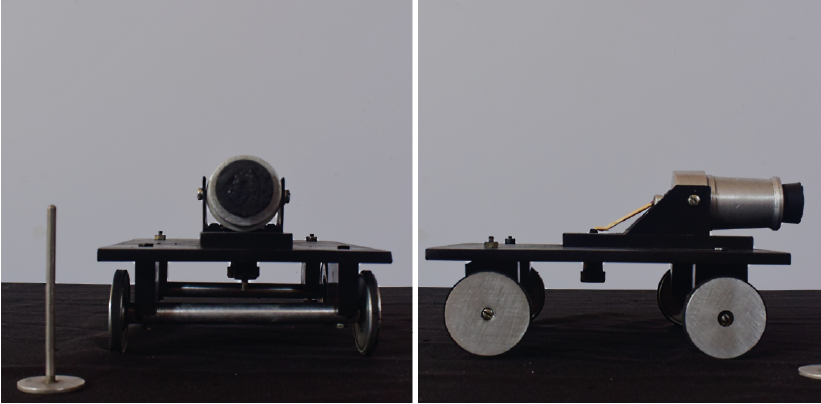
\includegraphics[width=1\linewidth]{cannon-1.png}
	\caption{Демонстрация  закона сохранения импульса}
	\label{cannon-1}
\end{figure}


\subsection*{\underline{Оборудование:}}

\begin{enumerate}
	\item Тележка с прикрепленной к ней пушкой
	\item Дымный порох
	\item Резиновая пробка, выполняющая роль снаряда
	\item Штатив с экраном (для торможения вылетевшего снаряда)
	\item Буфер для торможения откатившейся пушки
	\item Спички
\end{enumerate}

\newpage
\subsection*{\underline{Основные определения:}}

Третий закон Ньютона может быть записан через импульс и импульс силы.
Предварительно для изолированной системы, состоящей из двух тел с массами $ m_1 $ и $ m_2 $, имеющих начальные скорости $ \textbf{v}_1 $ и $ \textbf{v}_2 $ необходимо получить связь между скоростями $ \textbf{u}_1 $ и $ \textbf{u}_2 $, которые приобретут тела после взаимодействия с силами $ \textbf{F}_1 $ и $ \textbf{F}_2 $. 
Так как эти силы равны по модулю и противоположны по направлению, т. е. $ \textbf{F}_{1} = - \textbf{F}_{2} $, а также действуют между телами в течение одинакового времени $ \Delta t $, следовательно, 
$$
\textbf{F}_{1}\Delta t  = - \textbf{F}_{2}\Delta t .
$$

Уравнение (\ref{-}) можно переписать в виде
$$
m_1\textbf{u}_1 - m_1\textbf{v}_1 = - \left( m_2\textbf{u}_2 - m_2\textbf{v}_2 \right) .
$$

Слагаемые в уравнении (\ref{--}) удобно сгруппировать следующим образом:
$$
m_1\textbf{v}_1 + m_2\textbf{v}_2 = m_1\textbf{u}_1 - m_2\textbf{u}_2.
$$

Оказывается, что сумма импульсов тел изолированной системы остается постоянной 
при любых взаимодействиях тел.
Это же можно выразить и другими словами: 
\textit{\begin{flushleft}
		количество движения изолированной системы тел остается постоянным во все время движения системы: 
\end{flushleft}}
$$
m_1\textbf{v}_1 + m_2\textbf{v}_2 = \text{const}.
$$

Это утверждение называется законом сохранения импульса. 
Этот закон можно рассматривать как новое выражение третьего 
закона Ньютона.
Но теперь он связывает не значения самих сил, 
а устанавливает связь между конечными результатами действия 
этих сил. 

Отметим, что закон сохранения импульса в такой же форме можно применять и к некоторым неизолированным системам. 
Допустим, что на два тела, входящие в систему, кроме внутренних 
сил, действуют еще и внешние силы $ \textbf{F}_1 $ и $ \textbf{F}_2 $. 
Но силы $ \textbf{F}_1 $ и $ \textbf{F}_2 $ таковы, что их сумма равна нулю: 
$$
\textbf{F}_1 +  \textbf{F}_2 = 0
$$

Последнее условие означает, что будет равна нулю и 
сумма импульсов этих сил.
Повторяя рассуждения, можно показать, что для неизолированной системы 
тел будет справедливо следующее утверждение: 
\textit{\begin{flushleft}
		если сумма импульсов внешних сил равна нулю, то полный импульс системы тел не изменяется. 
\end{flushleft}}

Если же сумма импульсов внешних сил не равна нулю, то импульс системы должен меняться. 
Это изменение будет равно сумме импульсов внешних сил.

Закон сохранения импульса объясняет такие явления, как реактивное движение, отдачу (или откат) при выстреле, работу гребного винта или весел и другие.
Например, если рассматривать ружье и пулю как одну систему, то давление пороховых газов при выстреле будет для этой системы силой внутренней и не может изменить импульс системы, равное до выстрела нулю. Поэтому, сообщая пуле импульс $ m_{1}v_{1} $, направленное к дульному срезу, пороховые газы сообщат одновременно ружью численно такое же, но противоположно направленное импульса $ m_{2}v_{2} $, что вызовет отдачу; из равенства  $ m_{1}v_{1} = m_{2}v_{2} $ (где $ v_{1} $ , $ v_{2} $ — численные значения скоростей) можно, зная скорость $ v_{1} $; пули при вылете из ствола, найти наибольшую скорость $ v_{2} $ отдачи (а для орудия — отката).

\newpage
\subsection*{\underline{Краткое описание демонстрации:}}

Ствол пушки заполняется дымным порохом, после чего дуло плотно закрывается резиновой пробкой (рис.\ref{cannon-1}), служащей снарядом.
С задней стороны ствола пушки располагается фитиль представленный в виде спички.
За счет воспламенения фитиля загорается порох внутри пушки.
После взрыва резиновая пробка вылетает из пушки, а пушка откатывается назад (рис.\ref{cannon-2}).

\begin{figure}[H] 
	\centering 	
	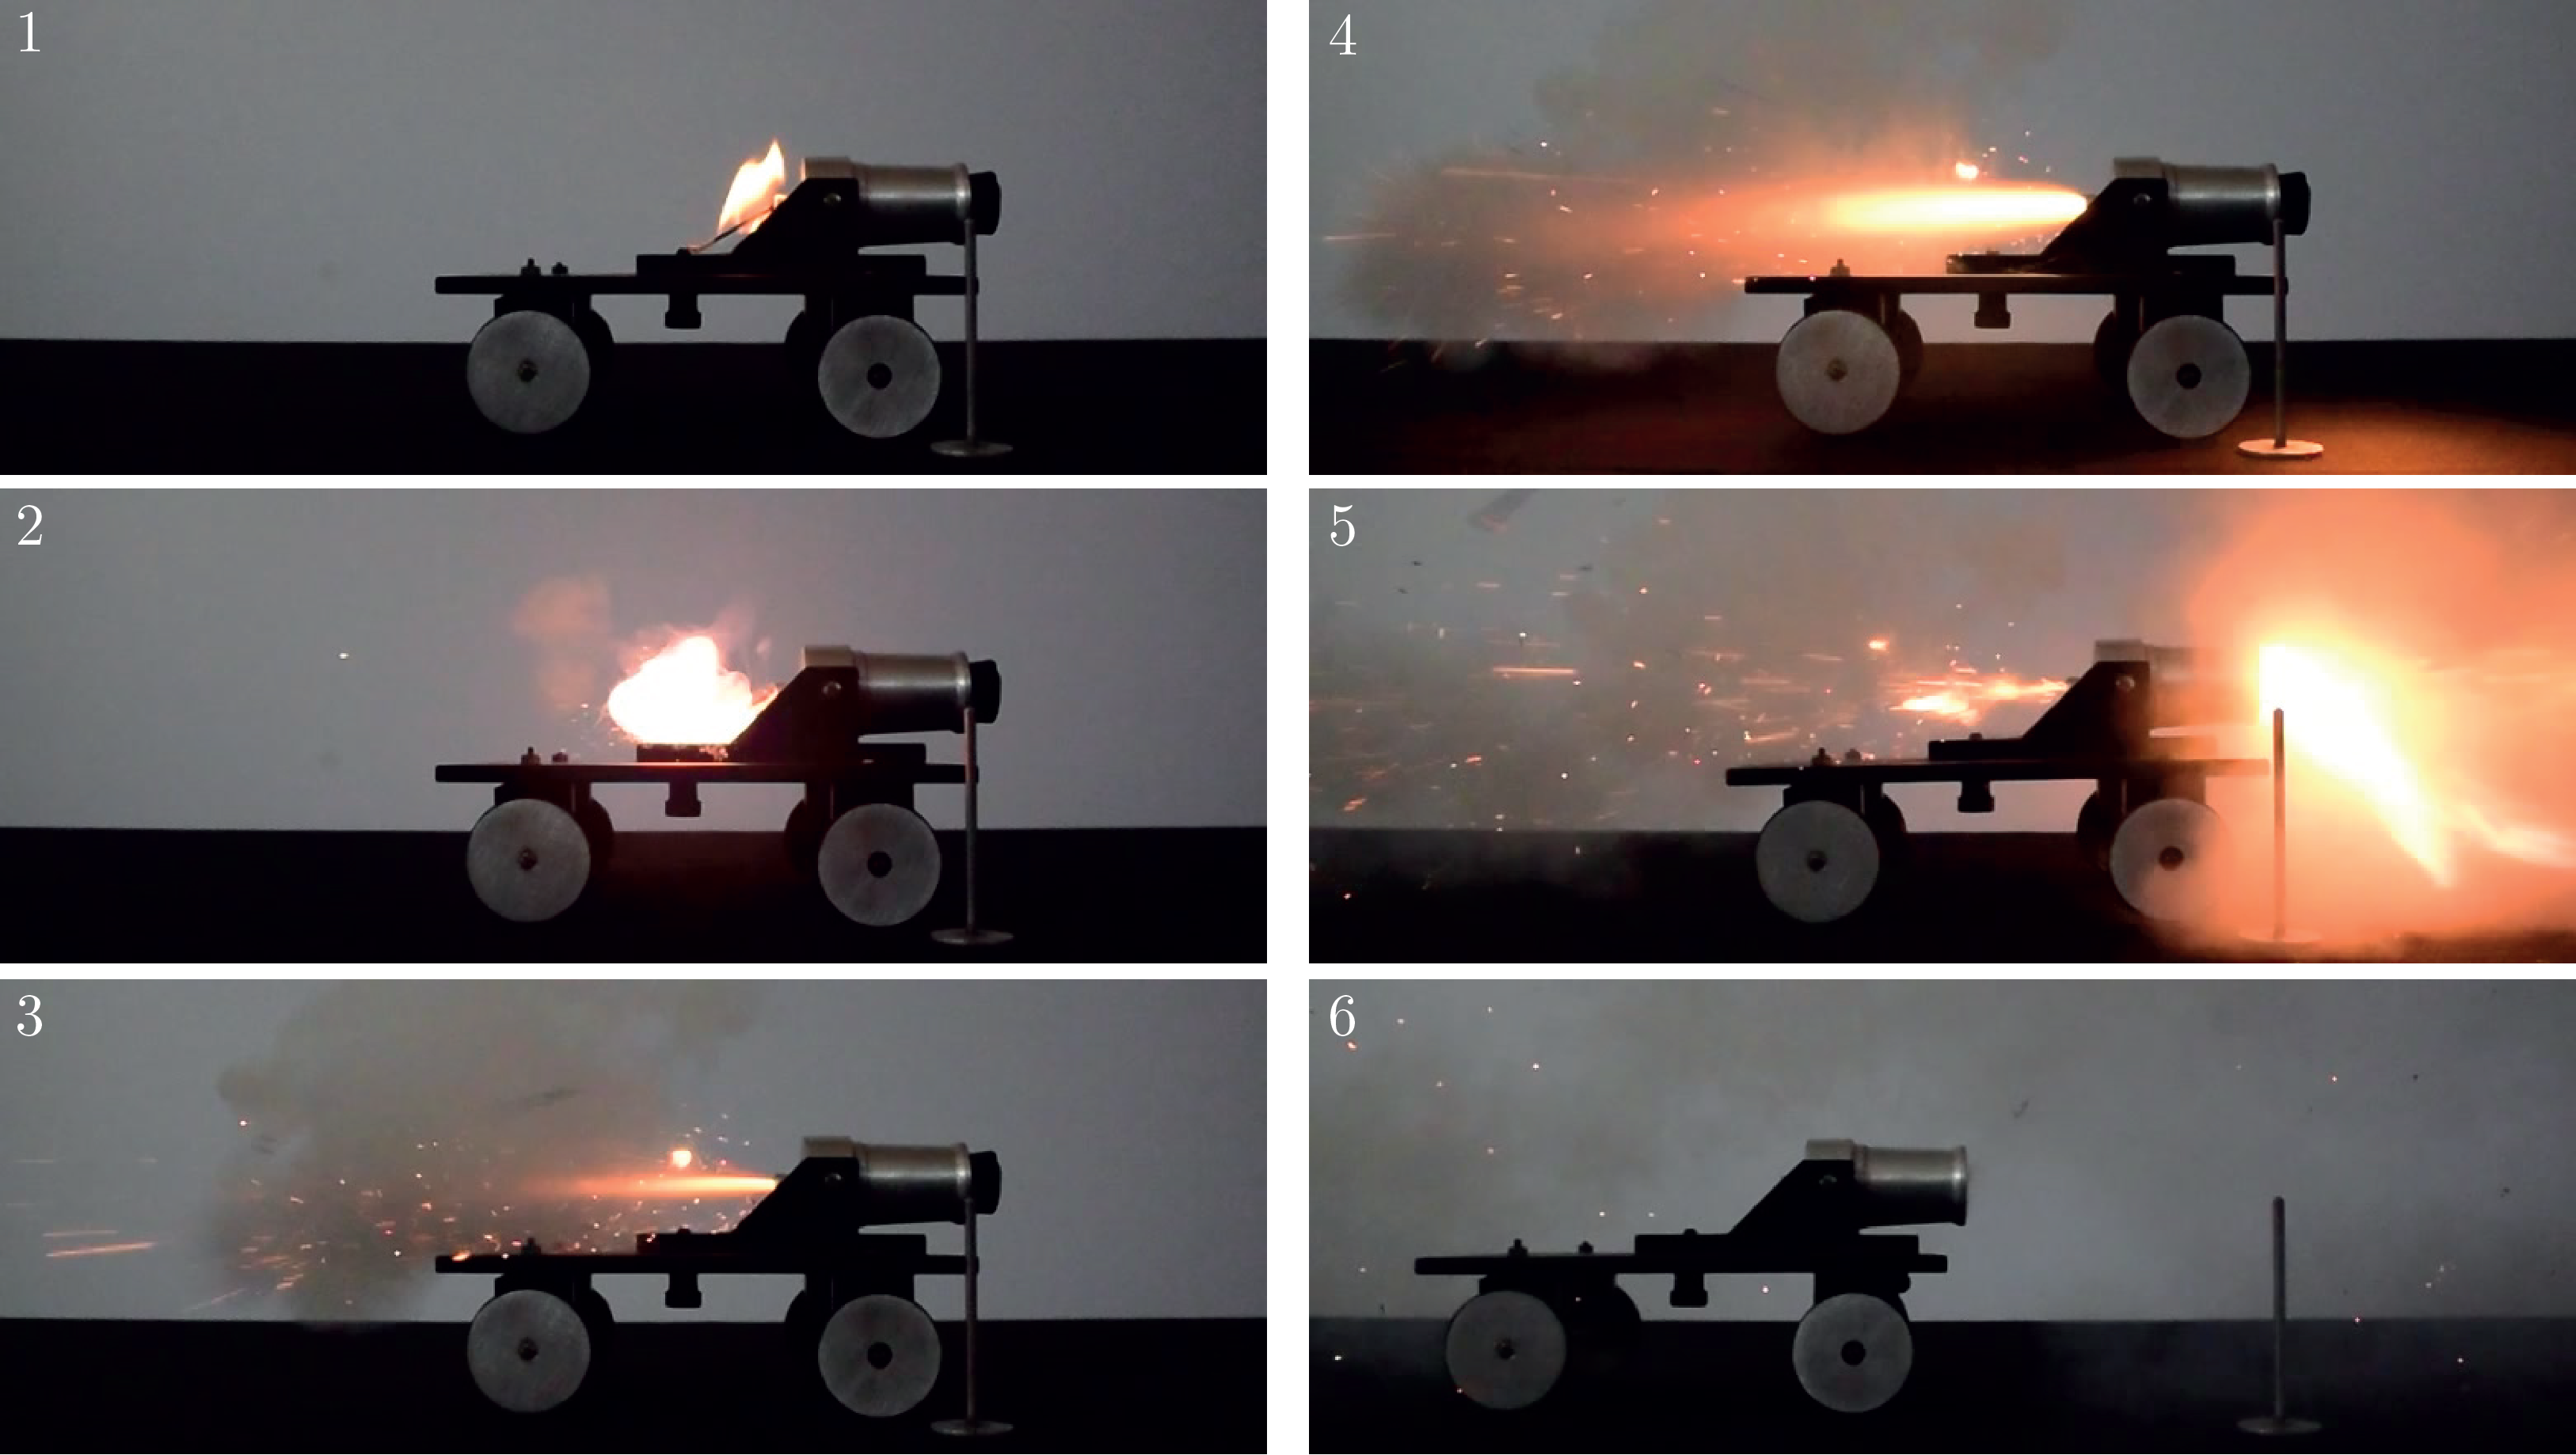
\includegraphics[width=0.9\linewidth]{cannon-2.png}
	\caption{Покадровое изображение поведения пушки при выстреле}
	\label{cannon-2}
\end{figure}

Данный опыт показывает, что импульс пушки и снаряда равны по величине, но противоположны по направлению.
Таким образом, в данном опыте наглядно показано выполнение закона сохранения импульса (скорости объектов обратно пропорциональны их массам, а их направления противоположны).

\newpage
\subsection*{\underline{Теория:}}

Снаряд и пушка являются замкнутой системой, для которой выполняется закон сохранения импульса. 
В результате выстрела из пушки, импульсы пушки и снаряда изменются.
Сумма же импульсов пушки и находящегося внутри снаряда до выстрела равна сумме импульсов откатывающейся пушки и летящего снаряда после выстрела.

Закон сохранения импульса для данной задачи имеет вид 
\begin{equation}\label{cannon-eq1}
 \textbf{P}_{\text{до}} = \textbf{P}_{\text{после}}
\end{equation}
где $ \textbf{P}_{\text{до}} $ — суммарный импульс до выстрела, а $ \textbf{P}_{\text{после}} $ — импульс после выстрела. 
\begin{equation}\label{cannon-eq2}
\textbf{P}_{\text{до}} = (m_{1} + m_{2})\textbf{v}_{1}
\end{equation}
где $ m_{1} $ — масса пушки, $ m_{2} $ — масса снаряда, $ \textbf{v}_{1} $ — скорость до выстрела.
Так как до выстрела пушка со снарядом покоилась, то можно записать: 
\begin{equation}\label{cannon-eq3}
\textbf{P}_{\text{до}} = (m_{1} + m_{2})\textbf{v}_{1} = 0
\end{equation}

\begin{equation}\label{cannon-eq4}
\textbf{P}_{\text{после}} = m_{1}\textbf{v}_{2} + m_{2}\textbf{v}_{2} 
\end{equation}
где $ \textbf{v}_{2} $ — скорость пушки после выстрела, $ \textbf{v}_{2} $ — скорость снаряда после выстрела.

\end{document}